\documentclass{article}
\usepackage{arxiv}
\usepackage[utf8]{inputenc}
\usepackage[english, russian]{babel}
\usepackage[T1]{fontenc}
\usepackage{url}
\usepackage{booktabs}
\usepackage{amsfonts}
\usepackage{nicefrac}
\usepackage{microtype}
\usepackage{lipsum}
\usepackage{amsmath}
\usepackage{color}
\usepackage{graphicx}
\usepackage{natbib}
\usepackage{doi}



\title{Polarization and neutrality detection of texts in the news flow}

\author{Роман Авдеев \\
	Студент 4 курса 417 гр.\\
	Факультет ВМК\\
        Кафедра ММП\\
	МГУ имени М. В. Ломоносова \\
	\texttt{roma.avdeyev@gmail.com} \\
	%% examples of more authors
	\And
	Константин Вячеславович Воронцов\\
        Профессор РАН, д.ф.-м.н., проф., зав.каф.ММП\\
	Факультет ВМК\\
        Кафедра ММП\\
	МГУ имени М. В. Ломоносова \\
	%% \AND
	%% Coauthor \\
	%% Affiliation \\
	%% Address \\
	%% \texttt{email} \\
	%% \And
	%% Coauthor \\
	%% Affiliation \\
	%% Address \\
	%% \texttt{email} \\
	%% \And
	%% Coauthor \\
	%% Affiliation \\
	%% Address \\
	%% \texttt{email} \\
}
\date{}

\renewcommand{\shorttitle}{\textit{arXiv} Template}

%%% Add PDF metadata to help others organize their library
%%% Once the PDF is generated, you can check the metadata with
%%% $ pdfinfo template.pdf
\hypersetup{
pdftitle={A template for the arxiv style},
pdfsubject={q-bio.NC, q-bio.QM},
pdfauthor={David S.~Hippocampus, Elias D.~Striatum},
pdfkeywords={First keyword, Second keyword, More},
}

\begin{document}
\maketitle

\begin{abstract}
	В данной работе предлагается способ определения поляризации текстов в новостном потоке. Решение основано на методах машинного обучения без учителя, что позволяет работать как с малыми, так и с большими наборами текстов. Решается задача разделения множества новостных сообщений на кластеры-мнения, выделения отдельных кластеров нейтральных и нерелевантных документов. Предложены метрики оценивания качества отсева нерелевантных и нейтральных сообщений.\\ Эксперименты проводились на датасете, состоящем из 30 корпусов новостных сообщений по темам «политика» и «происшествия».
\end{abstract}


\keywords{Поляризация \and sentiment analysis \and opinion mining \and нейтральность}

\section{Введение}
Задача кластеризации текстов (то есть разбиения множества документов на подмножества тематически близких) остается актуальной на протяжении ряда последних лет. Знания в этой области полезны не только для того, чтобы корректно идентифицировать мнения клиентов в отзывах на какой-либо продукт, но и для более сложных задач. Например, для сбора общественного мнения в рамках анализа ценообразования, конкурентной разведки, прогнозирования рынка, прогнозирования выборов и выявления рисков в банковских системах. \\

Решаемая мной проблема относится к областям Opinion Mining и Sentiment Analysis. В задачах первой упомянутой области происходит поиск (в блогах, форумах, интернет-магазинах и пр.) мнений пользователей о товарах и других объектах, а также производится анализ этих мнений. Вторая область близка к классической задаче контент-анализа текстов массовой коммуникации, в ней оценивается общая тональность высказываний и текста в целом.//
Cуществуют разные подходы к выявлению поляризации мнений в тексте. Многие из них основываются на работе нейронных сетей [10]. Также существует подход, при котором используется обучение с учителем, что не всегда является оптимальным из-за разного размера текстов и объема обучающей выборки в целом. Работы [1] и [3] базировались на тематическом моделировании. Их авторы используют такие модальности как SPO триплеты (subject-predicate-object), семанические роли (по Филлмору), тональность слов, социально-демографические показатели. Также было показано, что включение семантической близости текстов в модель улучшает качество, а социально-демографические показатели не вносят особого вклада.\\

В данной работе учтен опыт предыдущих работ, проведены эксперименты со структурой модели, с разными алгоритмами. Предложены метрики оценивания различных аспектов качества модели. 


\section{Данные}
Используемый датасет представляет собой набор из 30-ти корпусов новостных сообщений из рубрик <<Политика>> и <<Происшествия>>. В каждом корпусе от 8-ми до 33-х документов. Всего 452 документа.\\
\begin{figure}[!htb]
\center
    \includegraphics[width=0.7\textwidth]{docs_amount_in_corpuses.png}
    \caption{Количество документов в каждом корпусе}
\end{figure}
\textit{Разметкой} будем называть набор меток $X=\{x_1,...,x_n\}$, каждый элемент которого $x_i$ является меткой i-го сообщения в корпусе. Предполагается, что каждый корпус содержит сообщения об одном событии или теме, однако может содержать и посторонние сообщения. Метки $\{1,2,3,...\}$ соответствуют кластерам-полюсам общественного мнения по данной теме. Метка <0> означает, что сообщение является нейтральным, то есть не содержит субъективного мнения. Метка <-1> означает, что документ нерелевантен, то есть не относится к общей для всех сообщений теме.\\

Для разметки данного датасета использовался сервис Яндекс.Толока.

\section{Метрики}
Наша задача заключается в корректной кластеризации документов внутри каждой темы. Нужно не только верно выделить мнения, но и проверить, существует ли отдельная группа нейтральных/ нерелевантных документов. \\
Для сравнения разметки $X=\{x_1,...,x_n\}$ с «золотым стандартом» — экспертной разметкой $Y=\{y_1,...,y_n\}$, используются BCubed-версии точности и полноты поиска.\\
Для контроля качества алгоритма введем несколько критериев:\\

\textbf{\textcolor{blue}{Критерий М1: точность и полнота кластеризации мнений}}\\
Точность и полнота сначала определяются относительно каждого объекта $x_i$, затем усредняются по всем объектам с меткой мнения:\\

\hspace{4cm}$P =  \underset{x_i>0}{avr}P_i; \hspace{1cm} P_i = \frac{\sum_{k} [x_k=x_i \hspace{0.1cm} and \hspace{0.1cm} y_k=y_i]}{\sum_{k} [x_k=x_i]}$\\

\hspace{3.5cm}$R = \underset{y_i>0}{avr}R_i; \hspace{1cm} R_i = \frac{\sum_{k} [x_k=x_i \hspace{0.1cm} and \hspace{0.1cm} y_k=y_i]}{\sum_{k} [y_k=y_i]}$\\

(если знаменатель дроби оказывается равным нулю, то считается, что дробь равна нулю).\\
Агрегированный критерий (F1-мера) определяется как среднее гармоническое:\\ 

\hspace{5cm}$M_1(X, Y) = \frac{2PR}{P+R}$\\

\textbf{\textcolor{blue}{Критерий М2: точность и полнота отсева нейтральных документов}}\\
Определим точность и полноту отсносительно метки c (с=0):\\

\hspace{5cm}$P_c = \frac{\sum_{k} [x_k \neq c \hspace{0.1cm} and \hspace{0.1cm} y_k \neq c]}{\sum_{k} [x_k \neq c]}$\\

\hspace{5cm}$R_c = \frac{\sum_{k} [x_k \neq c \hspace{0.1cm} and \hspace{0.1cm} y_k \neq c]}{\sum_{k} [y_k \neq c]}$\\

Глядя на формулу, можно сказать, что по сути мы оцениваем, как хорошо модель отделяет субъективные позиции от нейтральной констатации фактов.
Агрегированный критерий (F1-мера) определения нейтральных сообщений:\\ 

\hspace{5cm}$M_2(X, Y) = \frac{2P_0R_0}{P_0+R_0}$\\

\textbf{\textcolor{blue}{Критерий М3: точность и полнота отсева нерелевантных документов}}\\
Здесь по аналогии с нейтральными документами мы оцениваем корректность выявления релевантных, отделяем нужные нам мнения от шума. Агрегированный критерий (F1-мера) определения релевантных сообщений (с=-1):\\ 

\hspace{5cm}$M_3(X, Y) = \frac{2P_{-1}R_{-1}}{P_{-1}+R_{-1}}$\\

\hspace{5cm}$M_4(X, Y) = \frac{min\{K_x, K_y\}}{max\{K_x, K_y\}}$\\
Обозначим через $K_x$ и $K_y$ число различных мнений в разметках X и Y соответственно.\\

\hspace{5cm}$M_4(X, Y) = \frac{min\{K_x, K_y\}}{max\{K_x, K_y\}}$\\


\subsection{Эксперименты с метриками}
Описанные выше метрики являются результатом нескольких экспериментов. Критерии M1 и M4 стабильно давали понятные и хорошо интерпретируемые результаты как для модели, так и для разметчиков. Проблемы возникали с M2 и M3. Количество найденных нерелевантных документов сильно отличается от корпуса к корпусу, но, как мы видим на рисунке №2, доля согласия у разметчиков довольно высокая. Сложнее ситуация обстоит с нейтральными документами. Во-первых, из рисунка №3 следует, что весь корпус документов может быть нейтральным (в отличие от нерелевантных). Во-вторых, доля согласия между асессорами существенно ниже.
\label{old_metrics}
Изначально точность и полнота для M2 и M3 задавались формулами:\\

\hspace{5cm}$P_c = \frac{\sum_{k} [x_k=y_k=c]}{\sum_{k} [x_k=c]}$\\

\hspace{5cm}$R_c = \frac{\sum_{k} [x_k=y_k=c]}{\sum_{k} [y_k=c]}$\\

При таком определении метрик возникало сразу несколько сложностей:
\begin{enumerate}
    \item неясно, как определять P в случае нулевого знаменателя, что случалось часто. Для precision нулевой знаменатель означает, что модель не нашла нерелевантные/нейтральные документы, что автоматически обнуляет и числитель дроби. Получили неопределенность вида $\frac{0}{0}$.
    \item аналогичная проблема возникает и с R. Нуль в знаменателе recall говорит о том, что в разметке нет нейтральных/нерелевантных документов. Тогда воникает вопрос, можем ли мы оценивать корпус для таких X и Y. При этом, оставив NaN и отказавшись от оценивания, мы теряем информацию о качестве модели.
    \item для М2 получаем очень низкие значения из-за довольно слабого согласия между экспертами.
\end{enumerate}
Результаты метрик при таком задании precision и recall представлены ниже:
\begin{table}[!htb]
\center
\begin{tabular}{|l|l|l|}
\hline
         & M2   & \multicolumn{1}{c|}{M3} \\ \hline
Разметка & 0.08 & 0.49                    \\ \hline
\end{tabular}
\end{table}\\

Оценим качество модели и уровень согласия разметчиков с помощью каппа-статистики Коэна: \\
$\kappa = \frac{p_0 - p_e}{1 - p_e}; \hspace{0.2cm} \kappa \in [0, 1]$, где $p_0$ - относительное наблюдамое согласие среди оценщиков (accuracy), $p_e$ - гипотетическая вероятность случайного совпадения.\\

Значения $\kappa$ носят следующий смысл (\cite{litlink11}):
\begin{table}[!htb]
\center
\begin{tabular}{|c|c|}
\hline
kappa        & интерпретация                              \\ \hline
\textless{}0 & согласие меньше, чем случайная вероятность \\ \hline
0            & нет согласия                               \\ \hline
0.1-0.2      & незначительное согласие                    \\ \hline
0.21-0.4     & "удовлетворительное" согласие              \\ \hline
0.41-0.6     & умеренное согласие                         \\ \hline
0.61-0.8     & существенное согласие                      \\ \hline
0.81-0.99    & почти идеальное согласие                   \\ \hline
1            & полное согласие                            \\ \hline
\end{tabular}
\end{table}
\newline
Применив данную метрику к нерелевантным документам, получил, что средний уровень согласия разметчиков - 0.35, а качество модели - 0.2. Вызвано это тем, что каппа-статистика сильно штрафует неверные ответы для класса с меньшим количеством объектов. Но от одного корпуса к другому <<меньшим классом>> может являться как множество нерелевантных/нейтральных, так и множество кластеров-мнений (см. рис.2 и рис.3). Таким образом, штрафы за ошибки разных типов <<смешиваются>>, и мы не получаем реальной оценки качества работы конкретного блока алгоритма. \\

Поэтому в качестве итоговых метрик были выбраны критерии, описанные в разделе \textcolor{cyan}{\ref{metrics}}.

\begin{section}{Модель}
\label{sentiment}
\subsection{Данные}
Опишем данные с технической точки зрения. На вход поступил JSON-файл, содержащий корпуса документов. Каждый документ имеет уникальный идентификационный номер. Также в имеющимся датасете присутствует текст каждой новости и выделенные именованные сущности с промаркированной тональностью.\\
Пример:  \verb|{'neg': {'ТАСС': 1, 'Приморском крае': 1}, 'pos': {'Орловской области': 1}}|\\

В ходе работы над моделью понадобились лемматизированные предложения, поэтому текст каждого документа был соответствующим образом обработан и добавлен в датасет.
\subsection{Эксперименты}
Сначала была предпринята попытка решить поставленную задачу с помощью методов обучения с учителем. Использовался RandomForestClassifier, работающий на TF-IDF (term frequency - inverse document frequency) представлении лемматизированного текста. Лучшим результатом являлась F1-мера, равная 0.95 для кластеризации мнений и 0.67 для выделения нейтральных. Однако при уменьшении обучающей выборки и увеличении тестовой данные значения стремительно падали. От такого варианта реализации было решено отказаться, так как в общем случае нам неизвестен размер приходящего датасета; кроме того, в реальной задаче отсутствует разметка, поэтому supervised методы не подойдут.\\

Далее был сформирован общий вид модели - алгоритм, имеющий трехступенчатую структуру: на 1-ом шаге проводится отсев нерелевантных документов, на 2-ом - нейтральных, а на 3-ем шаге выполняется деление на кластеры-мнения.\\

\subsubsection{Выделение нерелевантных документов}
Выделение нерелевантных документов происходит при помощи подсчета семантической близости лемматизированных предложений в каждом документе. Для этого используется библиотека SpaCy с готовым пайплайном \verb|ru_core_news_sm| для русского языка; данный пайплайн обучен на текстах новостей. Так как семантическая близость считается для пар документов, получаем $C_{\verb|docs_amount|}^2$ пар. Как будет описано ниже, мы не используем семантическую близость всех пар сообщений. Проведя несколько экспериментов, было решено брать только 8 самых близких к конкретному документу сообщений. А характеристикой документа является среднее значение семантической близости его 8-ми соседей. Подробное описание данных экспериментов представлено ниже.\\

\textbf{\textcolor{blue}{OPTICS}}\\
Сначала было решено применить unsupervised метод OPTICS (Ordering Points To Identify the Clustering Structure). Можно сказать, что OPTICS является обобщением более известного DBSCAN. Есть несколько существенных отличий и особенностей:
\begin{enumerate}
    \item OPTICS строит дендрограмму по ближайшим соседям точек
    \item также внутри OPTICS строится график достижимого расстояния (расстояния до ближайшего соседа) от номера точки, а кластеры определяются как <<долины>> на графике
    \begin{figure}[!htb]
    \center
        \includegraphics[width=0.4\textwidth]{optics_reachability.png}
        \includegraphics[width=0.4\textwidth]{optics_valleys.png}
        \caption{Принцип работы OPTICS}
    \end{figure}
    \item как и DBSCAN, OPTICS выделяет шумовые точки
    \item технология OPTICS требует больше памяти, так как хранит большое количество расстояний до ближайших точек для определения расстояния достижимости
    \item главным достоинством метода OPTICS является то, что он не требует указания параметра epsilon, что приводит к существенному сокращению процесса настройки параметров
\end{enumerate}

Данный подход дал следующие результаты:
\begin{table}[!htb]
    \center
    \begin{tabular}{|c|c|}
    \hline
             & M3*   \\ \hline
    Алгоритм & 0.39 \\ \hline
    Разметка & 0.49 \\ \hline
    \end{tabular}
\end{table}\\
* - метрика M3 вычислялась как агрегированный критерий поиска НЕрелевантных (раздел \textcolor{cyan}{\ref{old_metrics}})\\

Далее было решено протестировать методы, ориентированные именно на выявление аномалий.\\

\textbf{\textcolor{blue}{IsolationForest}}\label{isolationforest}\\
Попробовал применить алгоритм Isolation Forest, используя разное число деревьев (\verb|n_estimators|).\\

Результаты при использовании финальной реализации метрики M3 (раздел \textcolor{cyan}{\ref{metrics}}):
\begin{figure}[!htb]
    \center
        \includegraphics[width=0.5\textwidth]{isolation_forest_new_m3.png}
        \caption{Зависимость качества выделения нерелевантных от числа деревьев}
\end{figure}\\
Максимальное значение M3=0.781 было достигнуто при \verb|n_estimators|=1500 (при $M3_{expert}=0.93$).\\

Видим, что в сравнении с OPTICS (по <<старой>> метрике) качество повысилось. Однако существенным недостатком Isolation Forest является то, что он предполагает наличие лишь \textbf{нескольких} аномалий, а, глядя на разметку, мы видим, что в корпусе может присутствовать до 79\% нерелевантных документов. Поэтому было принято решение протестировать еще одну модель.\\

\textbf{\textcolor{blue}{OneClassSVM}}\\
Данный алгоритм позволяет осуществить более точную настройку выделения аномалий, также здесь по умолчанию стоит ограничение в 50\% на долю выбросов среди всей выборки, но этот параметр можно указать любым.\\

Сначала проверим три бейзлайна с разными ядрами:
\begin{enumerate}
    \item \verb|'linear'| - линейное ядро
    \item \verb|'rbf'| - радиальная базисная функция
    \item \verb|'poly'| - полиномиальное ядро
\end{enumerate}

\begin{table}[!htb]
    \center
    \begin{tabular}{|c|c|l|l|}
    \hline
             & linear & rbf   & poly  \\ \hline
    M3 (old) & 0.562  & 0.45  & 0.58  \\ \hline
    M3 (new) & 0.68   & 0.632 & 0.682 \\ \hline
    \end{tabular}
\end{table}
 Видим, что два из трех бейзлайнов превышают <<старую>> экспертную метрику M3 (0.49), а при повышении точности (tol) разница становится еще больше. Рассмотрев подробнее метки объектов, был заметен очень низкий precision при высоком recall. Такие показатели доказывают, что данная метрика действительно некорректно отражает качество выделения аномалий. Таким образом, подтвердились проблемы, указанные в разделе \textcolor{cyan}{\ref{old_metrics}}, поэтому с текущего момента будем оценивать все модели только по новой реализации критерия M3 (раздел \textcolor{cyan}{\ref{metrics}}).\\

 Что касается новой версии критерия M3, то лучшее значение достигается при полиномиальном ядре. Постараемся подобрать некоторые другие гиперпараметры для улучшение качества.\\

 Попробуем найти оптимальную степень полинома:
\begin{table}[!htb]
    \center
    \begin{tabular}{|l|l|l|l|l|l|l|l|l|}
    \hline
    \multicolumn{1}{|c|}{} & \multicolumn{1}{c|}{1} & 2     & 3     & 4     & 5     & 6     & 7    & 8     \\ \hline
    M3                     & 0.666                  & 0.666 & 0.682 & 0.672 & 0.671 & 0.684 & 0.68 & 0.669 \\ \hline
    \end{tabular}
\end{table}

Заметим, что значения практически не отличаются(различие в пределах шума).\\

Теперь обратим внимание на другой важный гиперпараметр OneClassSVM. Параметр nu отвечает за верхний порог ожидаемой доли аномалий в датасете. По умолчанию он равен 0.5. Посмотрим на значение метрики M3 при разных nu:

\begin{figure}[!htb]
    \center
        \includegraphics[width=0.6\textwidth]{oneclasssvm_nu.png}
        \caption{Зависимость значения М3 от верхнего порога доли аномалий}
\end{figure}

Качество ожидаемо снижается при увеличении верхнего порога. В разделе \textcolor{cyan}{\ref{nonrelev_data}} было показано, что в данном датасете асессоры нашли около 10\% нерелевантных документов. Поэтому наиболее высокое качество достигается именно при таком пороге. Но, используя данную информацию, мы фактически пользуемся разметкой, поэтому введем модифицированный алгоритм выделения нерелевантных сообщений.\\

Что касается остальных гиперпараметров OneClassSVM, их подбор сильно зависит от конкретного датасета, и, так как мы решаем поставленую задачу в общем виде, их перебирать не будем.\\

\textbf{\textcolor{blue}{Модифицированный алгоритм}}\\
Сначала коротко опишем подготовку данных в предыдущих экспериментах. Как было сказано в начале текущего раздела, мы не используем значения семантической близости всех пар документов, хотя на начальных этапах был вариант алгоритма, где для каждого документа считалась сумма расстояний до всех остальных сообщений. Такая модель достигла значения M3=0.685 при полиномиальном ядре с degree=6 и nu=default. Такой подход можно существенно улучшить. Теперь будем брать некоторое число <<соседей>> (наиболее близких сообщений) и усреднять эти значения. \\

Схематично алгоритм выглядит так:
\newpage
\begin{figure}[!htb]
    \center
        \includegraphics[width=0.5\textwidth]{diagram_new.png}
        \caption{Обработка семантической близости пар документов}
\end{figure}\\

Теперь попробуем разбить данные на две части и анализировать их отдельно. Мы можем сразу выделить 50\% документов с наибольшими усредненными значениями семантической близости. Эти сообщения будем считать заведомо релевантными, так как если в корпусе находится более половины шумовых объектов, то, возможно, они и являются <<чистыми>> данными, а меньшая часть - это аномалии. Далее к 50\%  документов с меньшими показателями применяем OneClassSVM/Isolation Forest. Здесь использование Isolation Forest уже более корректно, так как поиск нерелевантных происходит в подвыборке, и проблема, описанная в \textcolor{cyan}{\ref{isolationforest}} (IsolationForest), становится не такой серьезной.\\

Посмотрим на значения M3 при разном числе \verb|"соседей"|:
\begin{figure}[!htb]
    \center
        \includegraphics[width=0.9\textwidth]{m3_neighb_forest_svm.png}
        \caption{Зависимость значения M3 от числа соседей}
\end{figure}\\

Из четырех рассмотренных моделей IsloationForest и OneClassSVM(nu=default) являются общими решениями, в то время как другие две вариации OneClassSVM используют информацию из разметки, но при этом демонстрируют более высокое качество.\\

Теперь рассмотрим случай, когда число соседей зависит от размера корпуса. На приведенном ниже графике \verb|n_docs| обозначает количество документов в корпусе.
\newpage
\begin{figure}[!htb]
    \center
        \includegraphics[width=0.9\textwidth]{m3_neighb_forest_svm_docs.png}
        \caption{Зависимость значения M3 от числа соседей}
\end{figure}

Заметим, что данный график фактически представляет собой усредненную и сглаженную версию предыдущего. Оптимальным по суммарным результатам четырех графиков является \verb|n_docs//3|. Наверное, для небольших корпусов сообщений такой подход будет работать хорошо, но для многочисленных блоков документов лучше брать фиксированное число соседей.

\subsubsection{Выделение нейтральных документов}
Нейтральный документ представляет собой текст без какой-либо субъективной позиции и/или эмоциональной окраски. Поэтому в качестве основного инструмента для определения сообщений такого вида было решено взять эмоционально окрашенные именованные сущности, имеющиеся в датасете (раздел \textcolor{cyan}{\ref{sentiment}}).\\

\textbf{Первый подход:} для каждого документа проверялось наличие/отсутствие эмоционально окрашенных слов. Если таковых не было обнаружено, то документ считался нейтральным. При данной стратегии M2=0.64.\\

\textbf{Второй подход:} теперь положительно и негативно окрашенные именованные сущности разделяются. Проверяется гипотеза, что сентименты разной эмоциональной окраски могут друг друга компенсировать. Тогда документ считается нейтральным, если такие слова отсутствуют или если их одинаковое количество на каждой полярности. В таком случае M2=0.65.
\section{Headings: first level}
\label{sec:headings}

\lipsum[4] See Section \ref{sec:headings}.

\subsection{Headings: second level}
\lipsum[5]
\begin{equation}
	\xi _{ij}(t)=P(x_{t}=i,x_{t+1}=j|y,v,w;\theta)= {\frac {\alpha _{i}(t)a^{w_t}_{ij}\beta _{j}(t+1)b^{v_{t+1}}_{j}(y_{t+1})}{\sum _{i=1}^{N} \sum _{j=1}^{N} \alpha _{i}(t)a^{w_t}_{ij}\beta _{j}(t+1)b^{v_{t+1}}_{j}(y_{t+1})}}
\end{equation}

\subsubsection{Headings: third level}
\lipsum[6]

\paragraph{Paragraph}
\lipsum[7]



\section{Examples of citations, figures, tables, references}
\label{sec:others}

\subsection{Citations}
Citations use \verb+natbib+. The documentation may be found at
\begin{center}
	\url{http://mirrors.ctan.org/macros/latex/contrib/natbib/natnotes.pdf}
\end{center}

Here is an example usage of the two main commands (\verb+citet+ and \verb+citep+): Some people thought a thing \citep{kour2014real, hadash2018estimate} but other people thought something else \citep{kour2014fast}. Many people have speculated that if we knew exactly why \citet{kour2014fast} thought this\dots

\subsection{Figures}
\lipsum[10]
See Figure \ref{fig:fig1}. Here is how you add footnotes. \footnote{Sample of the first footnote.}
\lipsum[11]

\begin{figure}
	\centering
	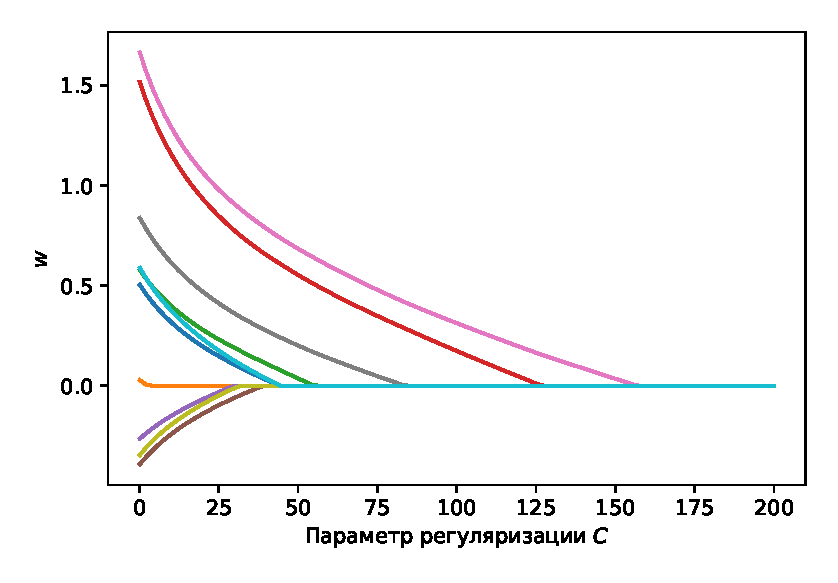
\includegraphics[width=0.5\textwidth]{../figures/log_reg_cs_exp.eps}
	\caption{Sample figure caption.}
	\label{fig:fig1}
\end{figure}

\subsection{Tables}
See awesome Table~\ref{tab:table}.

The documentation for \verb+booktabs+ (`Publication quality tables in LaTeX') is available from:
\begin{center}
	\url{https://www.ctan.org/pkg/booktabs}
\end{center}


\begin{table}
	\caption{Sample table title}
	\centering
	\begin{tabular}{lll}
		\toprule
		\multicolumn{2}{c}{Part}                   \\
		\cmidrule(r){1-2}
		Name     & Description     & Size ($\mu$m) \\
		\midrule
		Dendrite & Input terminal  & $\sim$100     \\
		Axon     & Output terminal & $\sim$10      \\
		Soma     & Cell body       & up to $10^6$  \\
		\bottomrule
	\end{tabular}
	\label{tab:table}
\end{table}

\subsection{Lists}
\begin{itemize}
	\item Lorem ipsum dolor sit amet
	\item consectetur adipiscing elit.
	\item Aliquam dignissim blandit est, in dictum tortor gravida eget. In ac rutrum magna.
\end{itemize}


\bibliographystyle{unsrtnat}
\bibliography{references}
\newpage
\addcontentsline{toc}{section}{Список литературы}
 
\begin{thebibliography}{}
    \bibitem{litlink1} Е.К.Милюта. \textit{Языковые модели для обнаружения поляризации общественного мнения в новостоном потоке}, 2022.
    \bibitem{litlink2} Большакова Е.И., Воронцов К.В., Ефремова Н.Э., Клышинский Э.С., Лукашевич Н.В., Сапин А.С. \textit{Автоматическая обработка текстов на естественном языке и анализ данных}, 2017.
    \bibitem{litlink3} Д.Г.Фельдман. \textit{Комбинирование фактов, семантических ролей и тональных слов в генеративной модели для поиска мнений}, 2020.
    \bibitem{litlink4} Kajal Yadav. \textit{Text Clustering using K-means}, 2021.
    \bibitem{litlink5} Francis Ndiritu. \textit{How to Build an NLP Based Emotion Detection Model using Neattext and Scikit-learn}, 2021.
    \bibitem{litlink6} Yasir Ali Solangi, Zulfiqar Ali Solangi. \textit{Review on Natural Language Processing (NLP) and Its Toolkits for Opinion Mining and Sentiment Analysis}, 2018.
    \bibitem{litlink7} Federico Pascual. \textit{Getting Started with Sentiment Analysis using Python}, 2022.
    \bibitem{litlink8} CY Yam. \textit{Emotion Detection and Recognition from Text Using Deep Learning}, 2015.
    \bibitem{litlink9} Enrique Amigo, Julio Gonzalo, Javier Artiles, Felisa Verdejo. \textit{A comparison of extrinsic clustering evaluation metrics based on formal constraints}, 2008.
    \bibitem{litlink10} Estela Saquete, David Tomás, Paloma Moreda, Patricio Martínez-Barco, Manuel Palomar. \textit{Fighting post-truth using natural language processing: A review and open challenges}, 2019.
    \bibitem{litlink11} Ajitesh Kumar. \textit{Cohen Kappa Score Python Example: Machine Learning}, 2022.
\end{thebibliography}

\end{document}